\documentclass[11pt,a4paper]{article} %title page
\usepackage[margin = 2cm]{geometry}


\usepackage{titletoc}
\usepackage[pagestyles]{titlesec}
\usepackage[no-math]{fontspec} 

%加這個就可以設定字體
\usepackage[CJKnumber, CJKchecksingle]{xeCJK} 
\usepackage[usenames,dvipsnames,svgnames,table]{xcolor}

\usepackage{paralist} % enhanced list environment
\usepackage{textcomp} % for including symbols
\usepackage{multicol} 
\usepackage{multirow}
\usepackage{threeparttable} %add footnote under tables
\usepackage{booktabs, tabularx} %extend control of width of columns 
%\usepackage{warpcol}%for decimal points alignment in tables


% packages about math
\usepackage{amssymb, amsmath, mathcomp} 

%for figs
\usepackage{placeins} % to flush all the floats before
\usepackage{graphicx}
\usepackage{wrapfig} %控制圖繞文 
\usepackage{float} % controlling the place of figure
\restylefloat{figure}

% for caption
\usepackage{caption, subcaption}
\usepackage{hyperref}

% for Reference
\usepackage[square, numbers, sort&compress]{natbib}
\usepackage[page,titletoc]{appendix} %toc for Appendices


%讓中英文字體分開設置
%設定中文的字型,可以直接輸入系統裡有的字型
\setCJKmainfont[BoldFont=DFHei Std W7]{DFHei Std W5}
\newCJKfontfamily{\kai}[BoldFont=DFKaiShu Std W7]{DFBiaoKaiShu Std W5}
\setmonofont[Mapping=tex-text]{Inconsolata}
%\setromanfont[Mapping=tex-text,BoldFont=Adobe Caslon Pro Bold]{Adobe Caslon Pro}
\setromanfont[Mapping=tex-text,BoldFont=Adobe Garamond Pro Bold]{Adobe Garamond Pro}
\setsansfont[Mapping=tex-text]{FuturaStd-Medium}
\newfontfamily{\optima}{OptimaLTStd}

\XeTeXlinebreaklocale "zh"
\XeTeXlinebreakskip = 0pt plus 1pt
%上面這二行,中文才能自動換行

\newcommand{\horrule}[1]{\rule{\linewidth}{#1}} 	% Horizontal rule
\newcommand{\nonumsubsec}[1]{\phantomsection \addcontentsline{toc}{subsection}{#1} \subsection*{\optima #1}}

\renewcommand{\thesection}{\Roman{section}}
\titleformat{\section}{\Large\bfseries}{\thesection.}{0.5em}{}
\renewcommand\figurename{圖}
\renewcommand\tablename{表}
%\renewcommand\lstlistlistingname{List of Source Codes}
%\renewcommand\lstlistingname{Code}


\newpagestyle{main}{\sethead{\small\kai\optima\sectiontitle}{\optima 2013 ML Final Project}{} \setfoot{}{\optima\thepage}{}\headrule}
%\newpagestyle{main}{\sethead{}{}{} \setfoot{}{\thepage}{}}

\renewcommand{\today}{\number\year 年 \number\month 月 \number\day 日}

%% Short-keys for easy typing
\newcommand{\figref}[1]{圖~\ref{#1}}
\newcommand{\tabref}[1]{表~\ref{#1}}

\newcommand{\scfi}[2] {\ensuremath{#1 \times 10^{#2}}}
\renewcommand{\t}[1]{\text{#1}}
\newcommand{\tk}{\text{k}}\newcommand{\tm}{\text{m}}
\newcommand{\tn}{\text{n}}\newcommand{\tM}{\text{M}}

\newcommand{\insertfig}[4]{\begin{figure}[H]
	\begin{center}
	\includegraphics[width = #2\textwidth]{#1}
	\caption{#3}\label{#4}
	\end{center}\end{figure}}
\newcommand{\insertfigx}[5]{\begin{figure}[#5]
	\begin{center}
	\includegraphics[width = #2\textwidth]{#1}
	\caption{#3}\label{#4}
	\end{center}\end{figure}}

\newcommand{\inserttable}[1]{
	\begin{table}[H]\vspace{-5pt}\begin{center}
	\input{#1}\vspace{-10pt}\end{center}\end{table}\vspace{-10pt}}
\newcommand{\inserttablex}[3]{
	\begin{table}[H]\begin{center}\caption{#2}\vspace{-10pt}\label{#3}
	\input{#1}\end{center}\vspace{-10pt}\end{table}}

%% end short-keys
\newcommand{\link}[2]{ \href{#1}{\textcolor{Gray}{#2}}}
\newcommand{\statatab}[1]{
\begin{table}[H]\centering\begin{threeparttable}
\input{#1}\end{threeparttable}\end{table}}

\usepackage{enumitem}
\usepackage{mathabx}


\pagestyle{main}
\begin{document}
%\setlength{\parindent}{0cm}
\setlength{\baselineskip}{1.5em}
\setlength{\parskip}{0.25em}

%%%%%% 抬頭 %%%%%%
\thispagestyle{empty}
\begin{center}
{\optima\LARGE Machine Learning Final Project}\\[0.5em]
電機五~王亮博~B98901114 \\
經研二~顏嘉儀~R01323019
\end{center}

%%%%% Workflow %%%%%%
\section{整理流程簡介}
基本上我們這組專注在 feature 的轉換與選擇,一開始是想透過選出比較有意義的 feature,也許用簡單的 model就能獲得不錯的準度。

\insertfigx{workflow/overview}{0.8}{整體處理流程}{fig:workflow-overview}{htb}

\figref{fig:workflow-overview} 所示即為本次整體的處理流程,能分成 Feature Selection 以及 Model Selection 兩大部份。透過 feature selection 之後,我們可以得到不同種方法產生的多個 feature space。之後就可以從這些 feature 中選出一部份來 train model。由於選用的 feature 可能會牽涉到高維度的轉換, $v_{dc}$ 的增加會讓我們有 overfitting 的問題,所以我們對此有兩個可以解決的方向:
\begin{enumerate}[itemsep=-1ex, topsep=0ex]
\item 在 model 選擇上,我們會盡量選擇 $v_{dc}$ 較低的演算法,例如 SVM、有 regularization 的 regression。
\item 為盡量減少最後選用 feature 的數目,可以考慮用 PCA 等方式降維。
\end{enumerate}

而在 Model Selection 我們使用 cross validation 的方式,找出最佳的參數組合,並重新以全部的資料 train,並上傳結果。以下便會針對 Feature Selection、Model Selection 作介紹,而實際在運作的過程中,我們也是將這兩部份拆開,分別完成。


%%%%%% Feature Selection %%%%%%%
\section{Feature Selection}
所有的操作皆在 Python 2.7/3.3 上進行。數值矩陣計算使用 Numpy 1.7+,而 SIFT 等跟影像計算有關的函式主要仰賴 OpenCV 2.4+/3.0-dev 版本,繪圖使用 matplotlib。

%%% FIG: Pixel view (raw and 60x60) %%%
\begin{figure}[htb]
    \centering
    \begin{subfigure}[b]{0.48\textwidth}
        \centering
        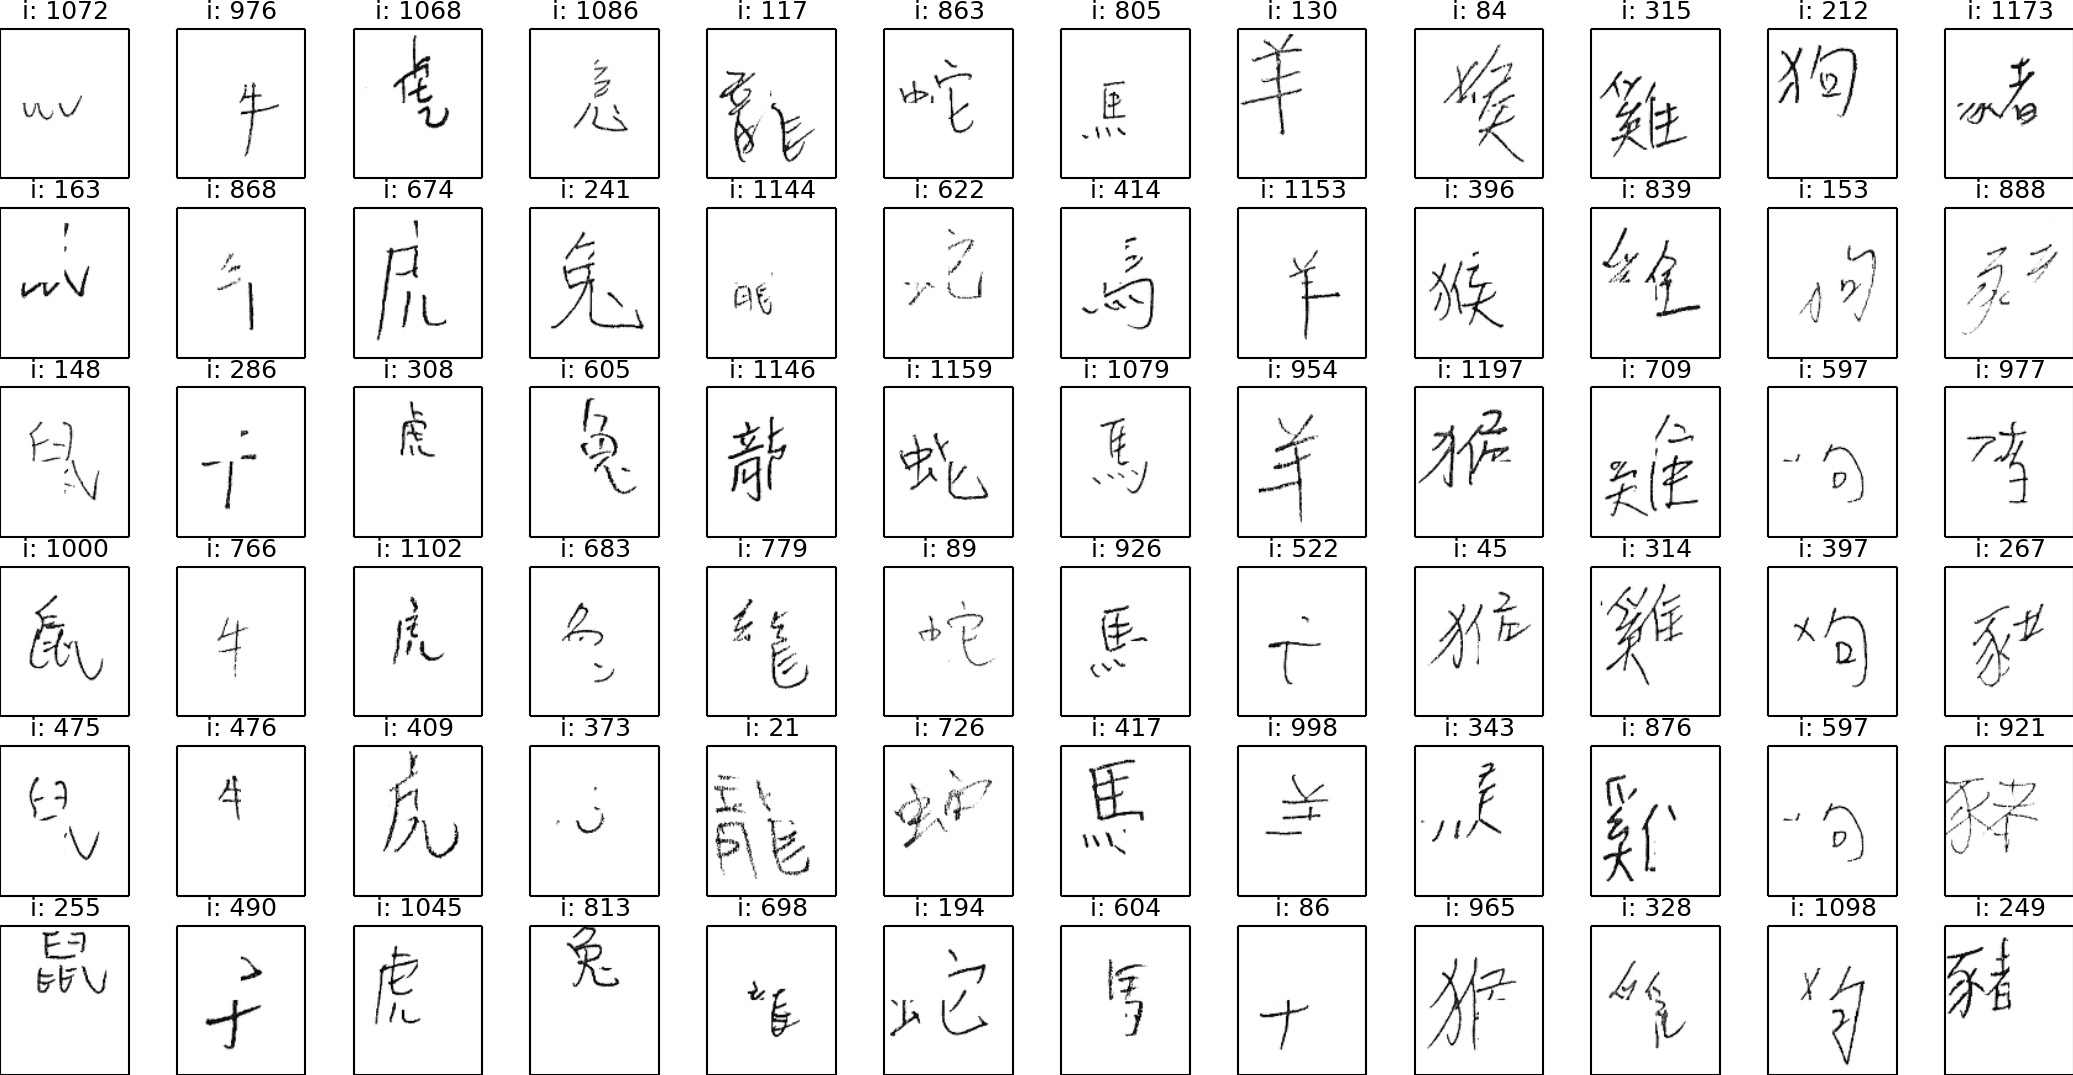
\includegraphics[scale=0.23]{../results/figs/train_pixelview_combined_6}
        \caption{Raw pixel input}
        \label{fig:px-raw}
    \end{subfigure}%
    ~
    \begin{subfigure}[b]{0.48\textwidth}
        \centering
        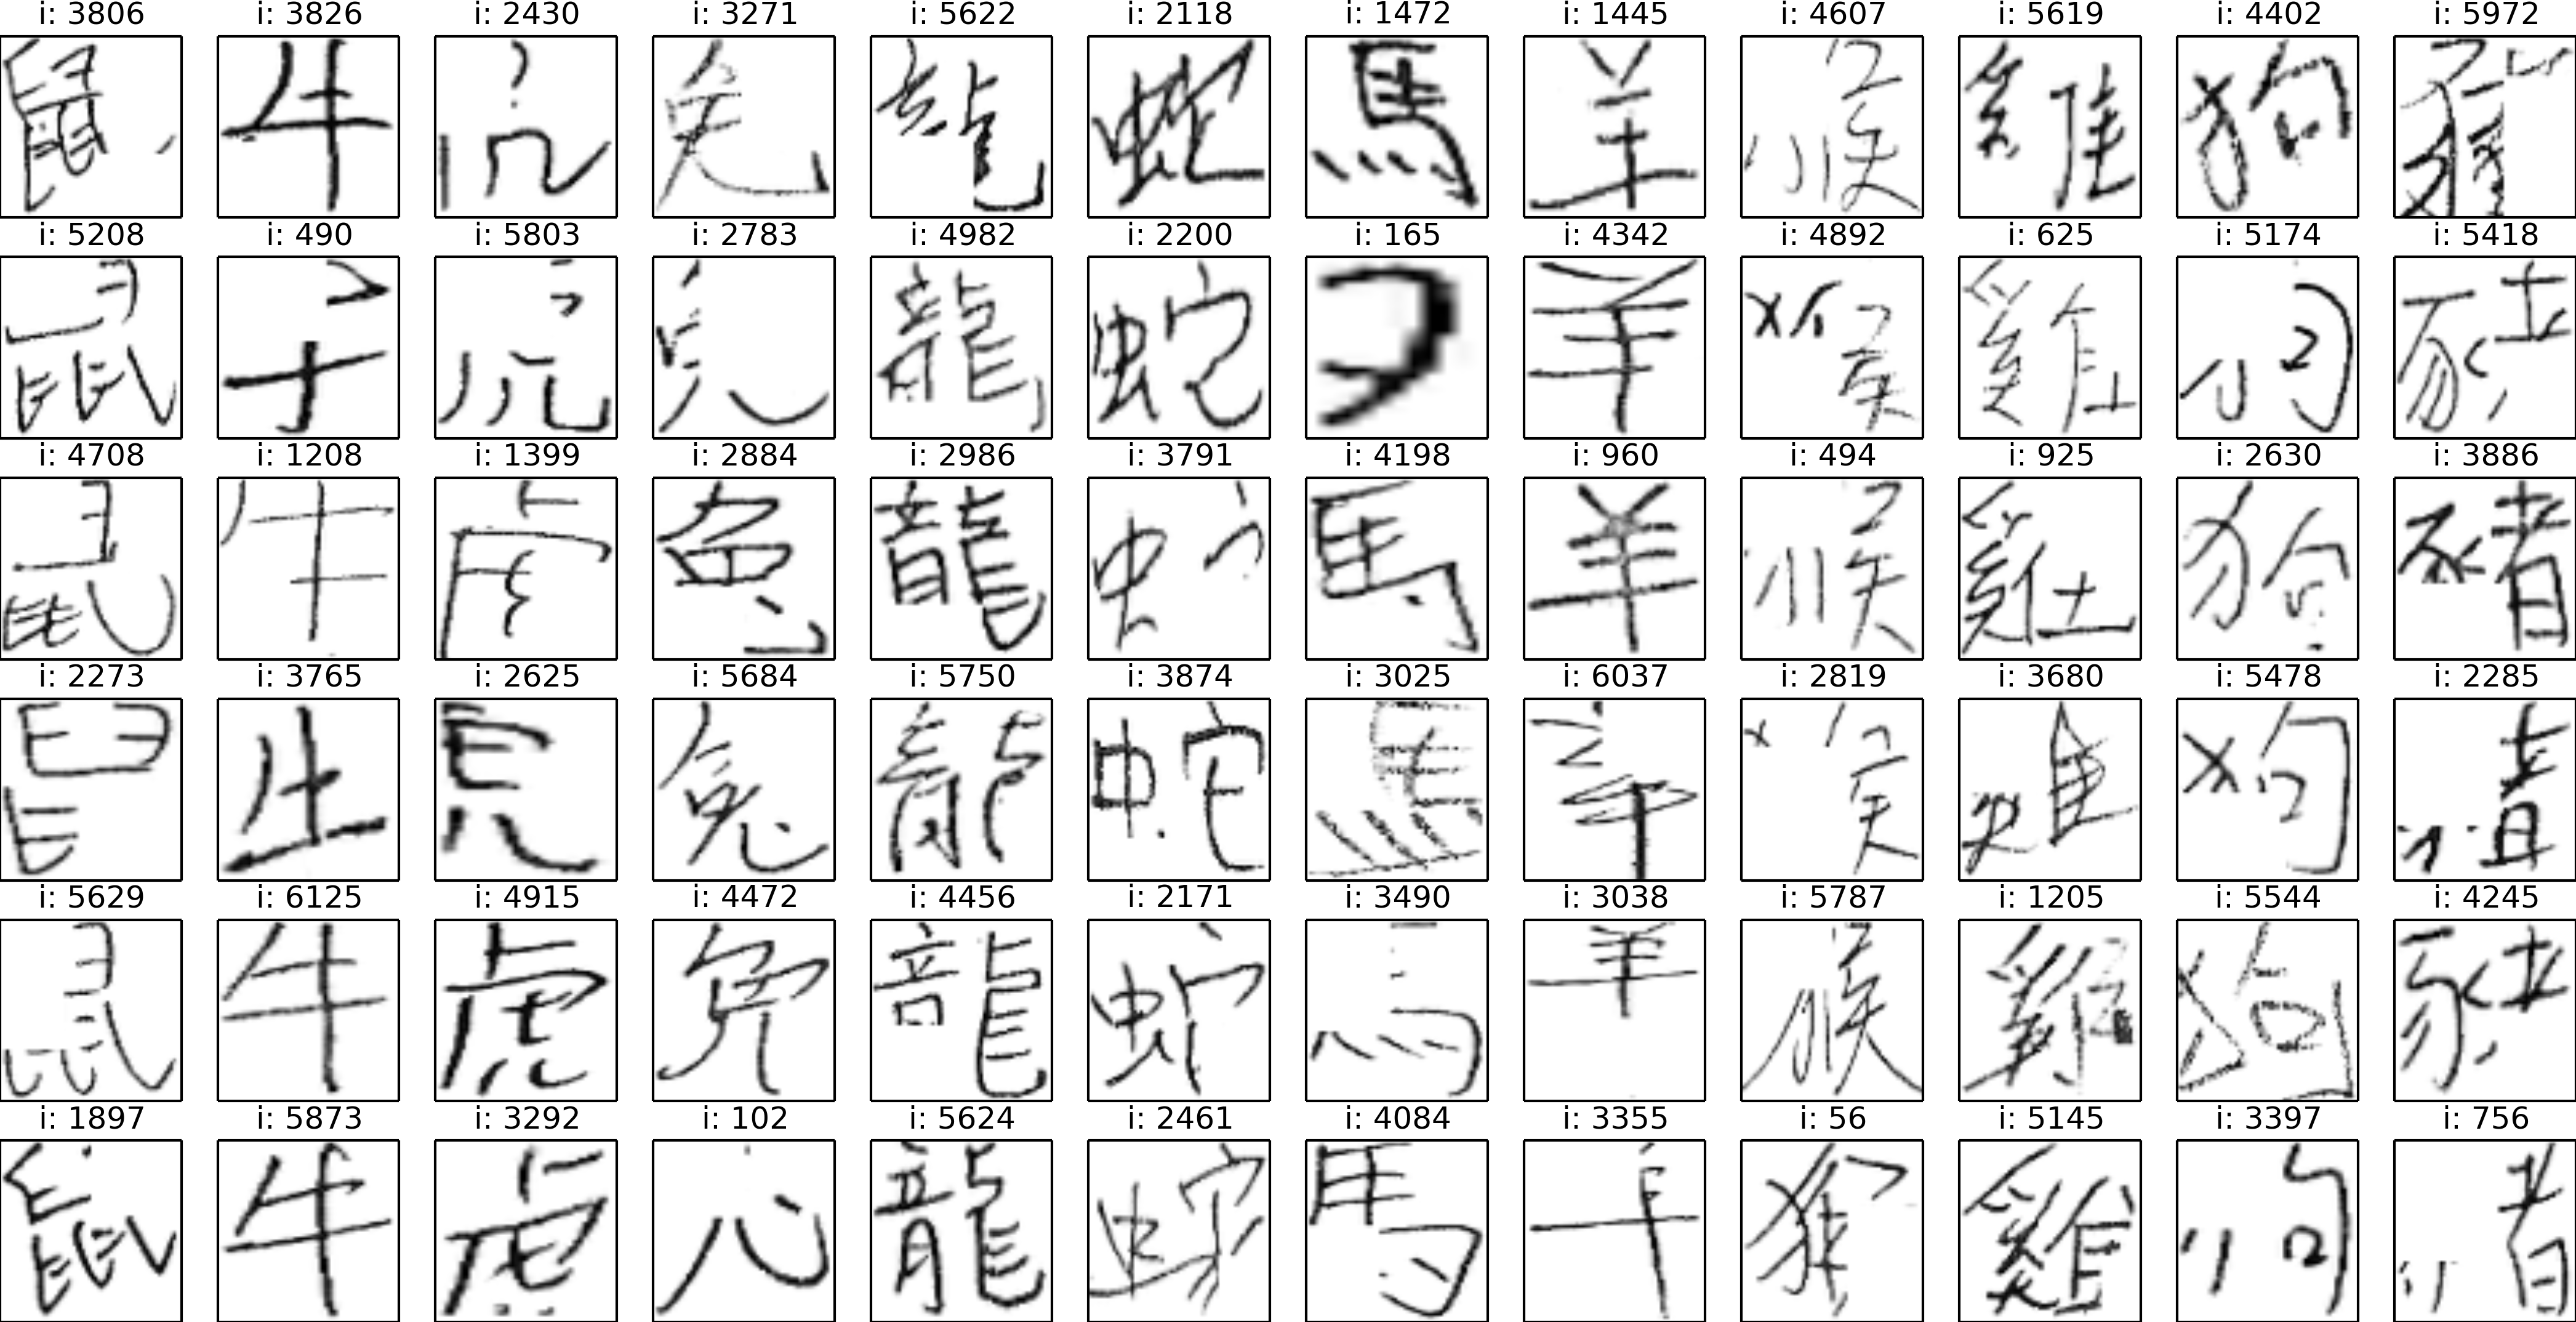
\includegraphics[scale=0.23]{../results/figs/train_pixelview_allzoidac_60x60_6}
        \caption{After 60x60 resize}
        \label{fig:px-60}
    \end{subfigure}
    \begin{subfigure}[b]{0.98\textwidth}
        \centering
        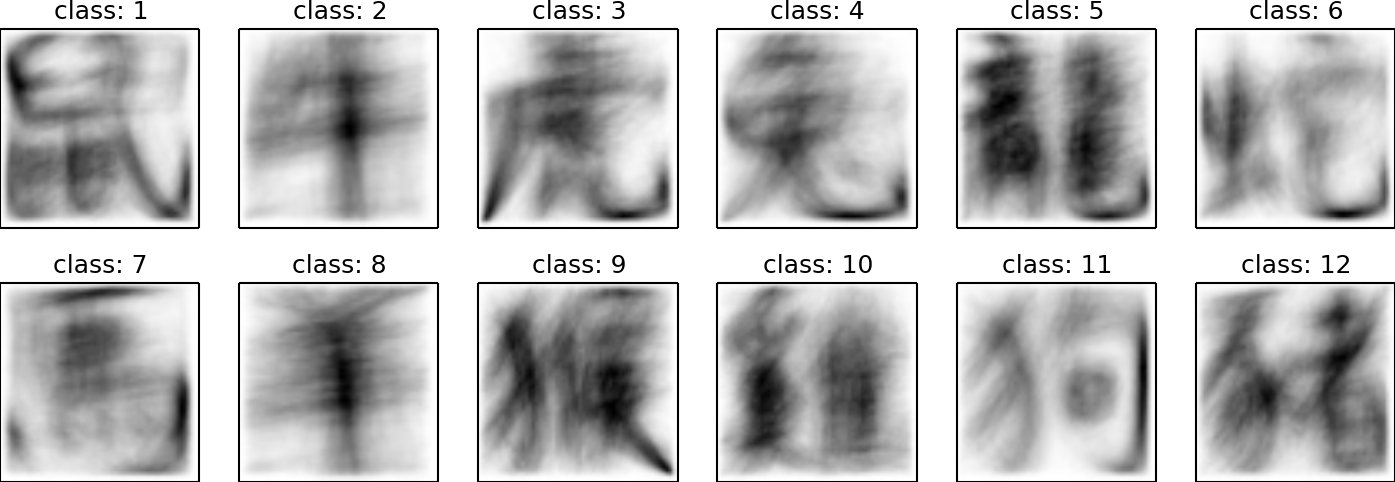
\includegraphics[scale=0.4]{../results/figs/60x60_avg}
        \caption{Aggregate mean of 60x60 resize data}
        \label{fig:px-60-mean}
    \end{subfigure}
    \caption{與 pixel 相關的 feature 概覽圖(可放大瀏覽)}\label{fig:px-overview}
\end{figure}

\subsection*{60x60 Resize}
首先預覽 data 樣貌,見\figref{fig:px-raw},發現每個字出現位置並非一致,如果直接將這 12,810 個 feature 去 train model 表現將不理想,我們實際跑也無法達到 50\% 以上的準確率。同時,由於 feature size 非常地大計算時間很長,但其實很多地方都是「空」的,一個字只佔用約 300 pixels 左右。因此我們第一個想解決的問題即是縮小 feature size,並且想辦法讓每個字都能大約在一樣的位置上,如此就能讓一個 pixel 的亮暗在整體上更具有意義,並且也能提昇計算速度。

我們選擇將原圖 resize 長寬皆 60 pixels,並且設定一個 threshold 將多餘的白邊的去除。60 僅是選一較原圖長寬小的值,同時在這大小 Linear SVM 每次可以在 5 分鐘內完成,故我們覺得這個大小合理便一直沿用下去,resize 結果可見 \figref{fig:px-60}。特例可參考 165(馬)、3038(羊) 等資料,因為在本來資料就有 1/4 遺失,resize 前者失去原有的空間特性(應該只是一個小小的勾),後者則是並沒有正確的將白邊去除。

當時初步認為這些資料屬於「較少數之例子」,故我們傾向直接忽視他們。對這些特例,前者可以藉由 resize 的比例來設定一個上限值,這樣以勾為例,就不會與正常馬的勾大小差距過多;後者則可以藉由二維的 histogram 來判斷畫素的分布是否跟該類別其他 data 差距明顯,或者再利用一個 threshold 較大的白邊去除器,如果畫素分布不均,在本例四邊切除之寬度差距會不等。

不過如果將轉換後的圖相疊做平均,見\figref{fig:px-60-mean},12生肖的字樣都能很清楚的浮現,這已較 raw 表現好,也達到起初目標。利用這樣的 feature 使用 RBF SVM 可以達到 7 成以上的準確度。這同時給了我們另一方向,因為往後考慮跟圖形特徵值辨識有關,在 raw 都有缺失資料的情況我們猜想即使是同組資料可能會有很不一樣的特徵值(例:剛好代表兩圖各缺失的角落),想要藉由將資料加上平均值來「還原回完整的字字」,再進行 model training,但以結論而言,由於 test data 並沒有這樣的特性,預測效果不理想。也有考慮直接用這 12 個字當 training,或再使用 OpenCV 中 Adaptive Threshold 方式抓出筆劃的外框,但同樣效果不彰。故最後放棄了這條方法。

\subsection*{SIFT 演算法(Scale Invariant Feature Transform)簡介}

% \insertfigx{workflow/SIFT_intro}{0.4}{SIFT descriptor gradient (DOG) 計算方式}{fig:sift-intro}{htb}

1999年, D.G.Lowe 提出SIFT 演算法\footnote{詳見``Object Recognition from Local Scale-Invariant Features'' (1999) 、``Distinctive Image Features from Scale-Invariant Keypoints'' (2004) 文章},主要用來處理影像的旋轉、放大縮小、亮度變化、視角變換。舉例來說,當我們說某人長得很有特色時(像是蒜頭鼻?),我們已經抓到這個人的特徵了,之後不管這個人換怎髮型、服裝,我們都不會認錯那隻蒜頭鼻。同理,影像也是,只要我們能找到影像的關鍵特徵,那即使這張圖放大縮小、旋轉,我們都可以認得他。

那接著問題就變成,該怎麼找到影像的關鍵向量。而透過 SIFT 的作法,能夠抓出這些特徵位置。他會尋找類似 blob 的點,即周圍亮中心暗或恰好相反這樣的模式。這即是找一個微分的 local max,但研究發現,用 Gaussian 一階導函數來對影像做 convolution ,不但能更快的算出微分值,同時選擇不同的 $\sigma$ 的 Gaussian,就好像在選擇不同大小的模式。因此只要除掉 $\sigma$ 的 scale,我們就可還原放大小縮小;而在方向上,他是選擇對應一個 patch 方格中,像素的 gradient 方向(大致上)。常見的結果顯示可見\figref{fig:sift-result}。


一旦有了每張圖的特徵向量,我們可以將兩張圖校正回同一個方向,並按照向量的長短,調整兩張圖到同樣大小,如上圖。套用到這次的資料,每個人寫的字大小且角度不一,藉由 SIFT 的幫助,有望反向校正回來。

\insertfigx{../results/figs/train_sift_allzoidac_60x60_}{0.9}{SIFT 特徵點標示示意圖。圖中每個圓圈皆為一個特徵點,橫線表該特徵點所代表之 patch gradient 方向,半徑大小與 $\sigma$ 有關,但實際 patch 較圓圈略大。}{fig:sift-result}{htb}


\subsection*{SIFT Datawise Pair Match}
這邊先對相關術語進行定義。每一筆資料 $i$,分別可能屬於 $Z=1,\ldots,12$ 生肖之一,$z$ 生肖擁有之總資料筆數定為 $I_z$。每筆資料 $i$ 經過 SIFT 後共有 $w_i$ 個特徵點 (visual word, VW),其第 $j$ 個特徵點對應之 gradient (descriptor) 為 $\mathbf{d}_{i, j}$。任兩個 VW 可以利用 $M(\mathbf{d}_a, \mathbf{d}_b)$ 來計算出 距離(相似度),距離越短表示兩 VW 越像。

當我想知道某個字 $i$ ($Z_i = 1$) 與 $Z=4$ 像不像時,我就把字 $i$ 對 $Z=4$ 中每個字求出以下的值:
\[
   \frac1{w_{i_z}} \sum_{
        \mathbf{d}_z \in \{ \mathbf{d}_{i_z, 1}, \ldots, \mathbf{d}_{i_z, w_{i_z}} \}
    }
    \left\ldbrack
        M(\mathbf{d}, \mathbf{d}_z) < th, ~ \forall \mathbf{d} \in \{\mathbf{d}_{i, 1}, \ldots \mathbf{d}_{i, w_i}\}
    \right\rdbrack
\]
也就是求出每個 $Z$ 中的字,他們有多少比例的 $\mathbf{d}$ 是有被字 $i$ 所吻合到的,並用一個 $th$ 閾值作判斷吻合。因此我們可得每一個生肖,這個吻合比例值的分布。如果今天是拿這筆資料所屬的生肖,理論上這裡面的字,會有較高比例的 $\mathbf{d}$ 特徵吻合,分布會較接近 1。最後選擇了前 150 ($K$) 高、20 個 quantile($Q$) 值、及整體的平均值來作 SIFT 轉換後的 feature。

這樣設計希望能平均地考慮同生肖字中每種寫法的的權重,例如有人馬的四點是連在一起,有些人沒有。但在全部的情況,只要這類的寫法有在 train 時出現,都可以被「某幾個字」所辨認出來,這群生肖的吻合比例值一樣會上升,反映在前 $K$ 高中。

但這個 feature 後來有幾個較嚴重的問題,第一他的計算時間很長,因為平均一個字有 30 - 60 個特徵點,兩兩特徵點計算,即便 SIFT 是個很快速的算法一樣需要花上很長的時間,也讓我們丟掉了第一階段上傳結果的機會…最後我們使用平行化 12 核情況下才讓它能在 3 小時左右算完。$th$ 本次考慮主要的調整參數,最後選用了 3 組 $th$。另一問題在於因為 train 保証自己的類別 TOP 1 特別高,但 test 並沒有這樣的特性,所以 cross validate 結果就很糟,有出現嚴重的 overfitting 情形。

不過我們對 SIFT 仍然深具信心!我們覺得主要問題在 SIFT 參數還可以做校調,同時,我們可以加入不等權重,把一些奇怪被蓋掉太多的字(可以用原始 pixel 數)來做 penalty。

\subsection*{SIFT Bag-of-Words Cluster}
有另一個做法是較多文獻所採用的 Bag-of-Words (BoW) 方式。這概念源自於文本主題分類時,首先我們一樣抓出每篇文章的關鍵字(VW),再來對這些關鍵字做 cluster,最後就用這 cluster 中的字來代表該主題。在本次生肖比對上就像有 12 個主題,只是在文章中,字只有出現/不出現兩種情況。而在 SIFT 中則是用一個 distance 來代表特徵點相似情況。

只要將 datawise 改成先對同生肖中,所有的特徵點 $\mathbf{d}$ (VW) 做,例如 \textit{k}-means 做 clustering,而這些 cluster 的中心點即是代表每個生肖的特徵點,train 時即對這些代表點做比對就好。如此可以大幅減少計算量,同時因為取得是代表生肖的中心點,相對也比較不受同生肖中奇怪的字影響,或者在 clustering 的時候這些怪字可能會自成一類,便可以標示出,另外做處理。

明明簡單修改,成效感覺顯著的方式為何不測?主是在我們對前面平行化的部份下了太多功夫,為了求快,我們簡化了許多計算步驟,同時我們後來又仔細看了一下結果,對「如何選擇 \textit{k}-means 的 \textit{k}」還有點疑慮,最後關鍵的時候,經討論後覺得我們應該要先花時間在 tune SIFT 相關的參數上,但可惜是我們賭錯了,算是本次 project 中很可惜的地方。

% \subsection*{Feature Transform Summary}

將四種可能的 feature 來源做表。
\begin{table}[htb]
\centering
\begin{threeparttable}
    \begin{tabular}{lrrrrrrrrr}
        \toprule
        Feature Set     & Raw           & 60x60 resize  & SIFT Datawise              & SIFT BoW \\
        \midrule
        \# features     & 12,810        & 3,600         & $N$ reduced to $12(K+Q+1)$ & $\sum W_z \approx 12W$\\
        Conversion Time & -             & fast (< 1min) & slow (> 20hr)              & fast (< 1hr)\\
        Training Time   & slow (20 min) & fast (< 5min) & fast (< 5min)              & fast (< 5min)\\
        \bottomrule
    \end{tabular}
\end{threeparttable}
\end{table}


%%%%%% Section: Model Selection %%%%%%
\section{Model Selection}
\subsection*{Neural Network}

\insertfigx{../report/workflow/NN_overview}{0.5}{Back-propagation Neural Network}{fig:NN-overview}{htb}

類神經網路和模糊理論一直是電腦視覺的領域裡的資優生,在指紋識別、衛星影像分析有很好的成績。因此當我們拿到這次的資料,很自然的就會想試試看類神經網路。類神經網路與其他模型相比,有許多優點:
\begin{enumerate}[itemsep=-1ex]
\item 良好的推廣能力(generalization) :對於未知的輸入也可以得到正確的輸出。
\item 可處理雜訊:對一個訓練好的網路而言,即使輸入有些缺值,依然有能力正確辨識。
\item 分散式結構,不易損壞:即使部份神經元損壞,整體仍然可以正常工作。
\item 可以很輕易的導入非線性模型。
\end{enumerate}
其中特點 1、2、3 相當讓人興奮,因為這正好呼應著我們這次的資料:每張圖片都有 1/4 的缺值。

我們決定從倒傳遞網路出發(Back-propagation Network),模型設定如\figref{fig:NN-overview}。倒傳遞網路最讓人困擾的就是參數設定,像是:隱藏層數量、神經元數量、訓練函數、次數、學習速率等。針對這個問題,我們採用「閃開!讓專業的來」策略,參考文獻以縮小參數範圍。

\begin{enumerate}[itemsep=-0.5ex, topsep=0ex]
\item 隱藏層數量:

根據 Villiers and Barnard (2002),設在 1、2 層之間有較好的收斂效果,多於兩層不利收斂且容易掉入局部最小值,不但耗時又招致較大誤差。我們實作發現,兩層效果較好。

\item 神經元數量:

根據 Piroska and Zaletnyik (1999),當樣本數足夠大時,選擇  35 個神經元即可有效描述輸入輸出關係,但仍需視樣本大小、耗費時間而定。我們選擇以試誤法決定數目。

\item 學習速率與慣性項:

過大的學習速率不利收斂,易導致震盪 ; 過小的學習速率則是收斂變慢,計算耗時。參考 Andrew Ng 的線上課程,我們決定使用較小的 learning rate,避免錯過最佳解。同時配合較大的慣性項,以避免落入局部最小值。最後我們決定學習速率設為 0.005,慣性設為 0.9。

\item  訓練次數、訓練比例:

參考 Stack Overflow 大大們的討論,通常訓練次數設在200左右,就有不錯的表現,太多則容易導致過度配適。關於 validation set 的比例,大大們提醒了一件事:確保你的 training set 具有足夠的代表性!更白話一點,小心拔掉的  validation set 使得  training set 改變分佈。從善如流,我們設定200次訓練、10\% validation set。

\item 樣本數與其他:

在訓練過程中,我們發現使用 6000 筆樣本進行訓練的結果,預測能力僅一成,幾乎等於亂猜。推測可能是樣本全開的  noise 量太多,反而學得不好。我們實驗性的使用小樣本,發現 600 個樣本點就有五成的預測力。最後,bias 項一定要記得打開,否則模型絕對不會收斂 !
\end{enumerate}

\begin{table}[htb]
\centering
\begin{threeparttable}
    \begin{tabular}{lrrrrrrrrr}
        \toprule
        no.&   sample&   Epoch&    學習速率&    慣性&   N1&   N2&       耗時&   $E_{in}$&  $E_{test}$\\
        \midrule
        1&     6144&    1000&   0.005&   0.9&   10&   10&   4h8m34s&   0.70&   0.88\\
        2&      615&    1000&   0.005&   0.9&   10&   10&    15m05s&   0.08&   0.43\\
        3&      615&     200&   0.005&   0.9&   10&   10&    14m07s&   0.07&   0.45\\
        3&      615&     200&   0.005&   0.9&   20&   20&    40m37s&   0.13&   0.51\\
        \bottomrule
    \end{tabular}
\end{threeparttable}
\end{table}

部份數據整理成上表。在簡單的設定下,類神經網路就顯著易於亂猜。但經過初步的嘗試後,我們發現類神經網路的缺點:
\begin{enumerate}[itemsep=-1ex, topsep=0ex]
\item 計算量非常大,訓練時間很長。
\item 對資料敏感,抽樣時要注意分佈有無平均。
\item 黑盒子,無法看出什麼是關鍵因子。
\item 參數的選擇無窮無盡,曠日耗時。
\end{enumerate}
缺點 1 與缺點 4 在硬體資源與訓練時間的壓力下,讓調整參數以獲得更好模型的方法,難以進行。我們決定將主力放在SVM的訓練上。

\subsection*{SVM}
我們使用 scikit-learn 的 LinearSVC 以及 RBF SVC (Gaussian Kernel) 來作 SVM 相關的 training。兩者能調整的參數很單純,即 $C, (\gamma)$ 兩種。例如我們會先決定 $\gamma = \{0.01, 0.1, 1, 10\}, C = \{1, 10, 100\}$ 等,就可以用他們所有的 combination 下去跑 3-fold CV,並找出 $E_{CV}$ 最低的參數值為何。底下的表格會其中之一的示例,使用 60x60 加上 mean 的 train 資料做 RBF SVM。

\begin{table}[htb]
\centering
\begin{threeparttable}
    \begin{tabular}{lrrr}
        \toprule
        $\gamma, \exp{-\gamma |x - x'|^2}$ & $C$ & $E_{CV}$ & $\sigma_{E_{CV}}$\\
        \midrule
        1&     100&   0.090  & 0.000\\
        0.1&   100&   0.090  & 0.000\\
        0.01&  100&   0.575  & 0.009\\
        0.001& 100&   0.970  & 0.001\\
        \bottomrule
    \end{tabular}
\end{threeparttable}
\end{table}

確定好範圍之後,可以再對參數做微調。但如果能有好的 feature,表示不同類別的差距很明顯,故此時不論用什麼參數,表現都不會差太多。除了$E_{CV}$ 值得參考外,每一類別的正確率與 support 數,以及記錄每一筆資料實際類別以及被預測類別的關系的矩陣 (Confusion Matrix) 都應該注意。不過大體上,SVM 的使用相當制式化。


\section{Performance Comparison}

最後,SIFT 類搭配 SVM 正確率與在 55\% 上下,反而是 60x60 搭配 SVM 表現最好,不但 $E_{CV}$ 與 $E_{test}$ 相近,正確率為 77\% 是我們試過方法中表現最好的。Neural Network 表現不好,推測是我們沒有太多時間在調整那些參數上,而且最後計算資源都賭在 SIFT 上面但表現不如預期。60x60 同前面描述是一個相當優良的 feature,所以我們後來也試跟與 SIFT 的結果一同搭配,但正確率並沒有提昇,而且 feature 多了近一倍,計算時間亦顯著變長。

我們後來有觀察到,其實關鍵很有可能是牛、羊的區別上。首先他們因為有缺資料的關系,例如只剩下半部,這肉眼幾乎分不出來。如果這兩類能區分開,正確率就能提昇。而特別針對 SIFT 的部份,牛羊因為筆劃結構很簡單,所以 SIFT 做 matching 時,幾乎別的類別的特徵點都有包含這「十」等部份,導致牛羊吻合率不論資料皆高,就很容易誤判。同時 SIFT 如果從 60x60 resize 開始做,表現也比 raw pixels 來得好。


\section{Conclusion}
對於這次的期末專題,我們的核心共識是:挑選好的 features 勝過挑選好的模型! 因此我們將力氣集中在資料的前處理上,希望能得到更好的 features。

在 features selection 方面,我們探索幾種可能的features transform,包括前面提到的:resized、對resized圖疊加取平均、實作SIFT。大體來說,轉換後的 features 都比原始資料來的好。
在 model selection 方面,我們選擇倒傳遞網路與SVM,作為我們的基本模型,在未調整參數的情況下,搭配 resized 的資料,預測力近五成,顯著異於亂猜。SVM 經過暴力搜尋最佳參數後,預測力可提昇至 77\%。

可惜的是,受限於硬體資源與時間,我們有太多發想,來不及實現。雖然結果未臻理想,但在這次實作的過程中,我們都學到很多 。再次感謝老師與助教們一學期以來的辛苦,感謝 !
\end{document}
